\documentclass[a4paper, 12pt]{report}
\usepackage[utf8]{inputenc}
\usepackage{graphicx}
\usepackage{hyperref}
\usepackage{xcolor}
\usepackage{titlesec}
\usepackage[left=2.5cm,top=2.5cm,right=2.5cm,bottom=2.5cm]{geometry}
\usepackage{moresize}
\usepackage{fontawesome5}
\definecolor{linkcolour}{rgb}{0,0.2,0.6}
\hypersetup{colorlinks,breaklinks,urlcolor=linkcolour,linkcolor=linkcolour}
\setlength{\parindent}{0pt}
\setlength{\parskip}{10pt}
\usepackage{tocloft}
\usepackage{tikz}
\usetikzlibrary{shapes.geometric, calc}
\usepackage{array}
\usepackage{dirtytalk}
\usepackage{ctable}
\usepackage{float}
\usepackage{hhline}
\usepackage[bottom]{footmisc}
\usepackage{booktabs}
\usepackage{multirow}
\usepackage{lmodern}
\usepackage{makecell}
\renewcommand{\thefootnote}{\dag}

\newcommand\rating[2]{%
  \pgfmathsetmacro\pgfxa{#1 + 1}%
  \tikzstyle{scorestars}=[star, star points=5, star point ratio=2.25, draw, inner sep=0.15em, anchor=outer point 3]%
  \begin{tikzpicture}[baseline]
    \foreach \i in {1, ..., #2} {
      \pgfmathparse{\i<=#1 ? "black" : "white"}
      \edef\starcolor{\pgfmathresult}
      \draw (\i*1.3em, 0) node[name=star\i, scorestars, fill=\starcolor]  {};
    }
    \pgfmathparse{#1>int(#1) ? int(#1+1) : 0}
    \let\partstar=\pgfmathresult
    \ifnum\partstar>0
      \pgfmathsetmacro\starpart{#1-(int(#1)}
      \path [clip] ($(star\partstar.outer point 3)!(star\partstar.outer point 2)!(star\partstar.outer point 4)$) rectangle 
      ($(star\partstar.outer point 2 |- star\partstar.outer point 1)!\starpart!(star\partstar.outer point 1 -| star\partstar.outer point 5)$);
      \fill (\partstar*1em, 0) node[scorestars, fill=yellow]  {};
    \fi
  \end{tikzpicture}%
}

% Adjust the line spacing in the Table of Contents
\setlength{\cftbeforesecskip}{8pt}  % Adjust spacing before sections
\setlength{\cftbeforesubsecskip}{8pt} % Adjust spacing before subsections
\setlength{\cftbeforechapskip}{15pt}

% Färg och rubrikformat
\definecolor{black}{RGB}{0, 0, 0}
\definecolor{myblue}{RGB}{45, 62, 80}
\definecolor{mygray}{RGB}{100, 100, 100}
\titleformat{\chapter}[hang]{\Huge\bfseries\color{black}}{\thechapter.}{20pt}{}
\titleformat{\section}[hang]{\Large\bfseries\color{black}}{\thesection}{12pt}{}
\titleformat{\subsection}[hang]{\large\bfseries\color{black}}{\thesubsection}{10pt}{}

\begin{document}
% Omslagssida
\thispagestyle{empty}
\vspace*{0.5cm}
\begin{center}
    {\Huge{\textbf{\noindent\hrulefill \hspace{1cm}Travel Report\hspace{1cm}\noindent\hrulefill}}} \\
    \vspace{0.5cm}
    {\large{\textsc{Nanyang Technological University (NTU) \\[0.1cm] SINGAPORE \\[0.2cm] Spring Term, 2025 \\[1cm]}}} 
    \begin{figure}[h]
        \centering
        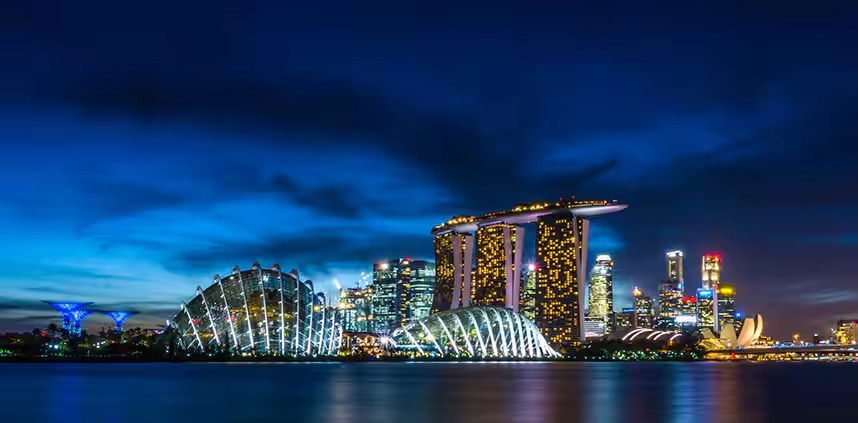
\includegraphics[width=0.99\linewidth]{figs/title_fig.jpeg}
    \end{figure}
\end{center}
{\Large \textbf{Oscar Stommendal}}
\vspace{-0.3cm}

\noindent\hrulefill

\textsc{B.Sc. Engineering Physics \hspace{0.15cm} $\vert$ \hspace{0.15cm} M.Sc. Physics (MPPHS) \\[0.2cm]
    Contact:} \begin{tabular}[c]{l l l}
    \hspace{0.15cm}
    \href{mailto:oscar.stommendal01@gmail.com}{\raisebox{-0.05\height}\faEnvelope \ \textsc{Email}} \hspace{0.15cm} $\vert$ \hspace{0.2cm}
    \href{https://linkedin.com/in/oscar-stommendal} {\raisebox{-0.05\height}\faLinkedin\ \textsc{LinkedIn}}
\end{tabular}
\\[-1cm]
\begin{center}
\noindent\hrulefill \\[1cm]
\textsc{\today}
\vfill
\begin{figure}[h]
    \centering
    
\includegraphics[width=0.8\linewidth, trim ={1.5cm, 3.5cm, 2.5cm, 3.5cm},clip]{figs/main_fig.pdf}
    \label{fig:title}
\end{figure}
\end{center}

\newpage
\tableofcontents
\thispagestyle{empty}
\newpage
\setcounter{page}{1}
\chapter*{Introduction}
\addcontentsline{toc}{chapter}{Introduction}


\chapter*{Preparations}
\addcontentsline{toc}{chapter}{Preparations}
\vspace{-0.6cm}
As you might understand, there is some preparation work you need to complete before travelling across the globe. However, just like my experience with Swedish and Chalmers culture, I found that Singapore and NTU as well are very well organized (except for the course selection process, which I'll address later). All the necessary steps in the application process were clearly outlined. I have friends who went to other countries where equivalent processes seemed less straightforward, from what I understood. Either way, I hope the following sections make the application process smoother and provide some additional useful tips and tricks. I wrote this as I completed each step to ensure the information was fresh in my mind. That said, keep in mind that things can change from year to year, so this guide should not be treated as the ``definitive truth''. Always follow the official instructions from NTU, and if you notice any discrepancies between my explanations and NTU's guidance, assume their version is correct. Lastly, note that the deadlines I mention below may differ depending on whether your exchange starts in the autumn or spring. 
\vspace{-0.25cm}
\section*{The Application Process}\label{app}
\phantomsection
\addcontentsline{toc}{section}{The Application Process}
I was nominated by Chalmers in early September and received an email from NTU shortly thereafter. As an Engineering Physics student, it was somewhat unclear to the Chalmers coordinator whether to nominate me to the College of Engineering (CoE) or the College of Science (CoS). Ultimately, another physics student and I decided that CoS suited us best. It was not entirely clear what being nominated to a specific college actually meant. From what I understood, the main requirement was to ensure that at least 50 \% of your course credits came from the college you were nominated to. However, I am not entirely sure this was checked in the end. Looking back, I am happy with my decision to be nominated to CoS as a Physics MSc student. I found that the most relevant courses for me were offered there (the other Chalmers students, e.g. from I or M, were nominated to CoE). For most MSc programs at Chalmers, I would assume CoE is the more appropriate choice, and it would likely work for Physics-related MSc programs as well. 

Additionally, whether you are nominated as a graduate or undergraduate student also comes with some catches. If given the choice, I would recommend asking to be nominated as an undergraduate (which I believe is the usual case). This allows you to apply for both postgraduate and undergraduate courses, which is not the case if you are nominated as a postgraduate student. As a postgraduate nominee, you will likely face challenges applying for undergraduate courses. Moreover, during my exchange term, there were not many postgraduate courses available to exchange students at all, which further supports being nominated as an undergraduate.

Going back to the application -- in the said email received after the nomination, NTU provided a link to the application portal together with accompanying instructions. Apart from some weird instances of queries, e.g. entering your ``race'', this form mostly asked for basic information: contact information, medical status and special needs etc. You also needed to provide a photo of the bio-data page in your passport (i.e. the pages with your photo, make sure to save this for later!) and a photo of yourself cropped to a specific size (also save this!). For the latter, I used a ``passport-photo-maker''-app (link \href{https://www.google.com/url?sa=t&source=web&rct=j&opi=89978449&url=https://apps.apple.com/se/app/passport-size-photo-maker-app/id1615533705&ved=2ahUKEwjq7fmg14eKAxXlIRAIHYyYDKcQFnoECEIQAQ&usg=AOvVaw2MFZUfJ5qukJls3hL6DmwZ}{here}), which seemed to work well. You also had to provide you English certificate (I received mine a couple of months earlier via my Chalmers email) and your transcripts of records (ToR).  Lastly, you were asked to enter 10 courses that you found interesting. You might hear otherwise, but to me, these only served as a ``check'' that you have done some research on the courses available -- you can easily swap freely among more courses later on (see \hyperref[courses]{Course Selection and Registration}).

Regarding the ToR, Chalmers Servicecenter started signing these electronically some time before our application deadline. However, NTU demanded these to have the Chalmers seal, which the electronic sign did not provide. Make sure to check if this is still the case for you! I know some students who did not want to wait for the coordinators to fix this, so they printed their ToR and went to Chalmers Servicecenter to get them signed. Thus, that is definitely an option to get them signed with the seal if the coordinators are slow for some reason. Overall, the instructions made the form rather easy and straightforward to complete, and if these were followed, your application was most likely approved.
\section*{After Being Accepted}
\addcontentsline{toc}{section}{After Being Accepted}
If you'd done everything correctly in your application, access to the Exchange/Study Abroad Portal (SAP) was granted in the beginning of November. This portal contains essentially everything you need to know and prepare prior to your exchange. There was also a pre-arrival meeting held on Teams in the second half of November. I would argue that, as I claimed, the portal itself provided all the necessary information, however the meeting was a nice way of hearing everything at once. Also, a link to a Telegram group was provided, where all incoming exchange students to NTU could ask each other questions about the application process. However, this later evolved into a great way to get in touch with potential travel partners or maybe find some people up for a beer.

Inside the portal, the first things you had to do before a deadline was to accept the NTU exchange offer, download the Letter of Enrolment (print this, since it will be needed when entering Singapore) and apply for campus housing (if you wanted). Regarding the housing, you can read more about my experiences under the \hyperref[housing]{Housing} section in the next chapter. After accepting the offer you could also activate your NTU Email and Network. From this point on, I would recommend (and I also believe that NTU does) that you use this email for all future communication with NTU in order to not end up as spam. Next, you had to apply and appeal for additional courses apart from the 10 chosen in your initial application and also submit your Student's Pass (STP) application. You can read more about this in the two following sections. Moreover, something I couldn't find explicitly stated in the SAP (at least not clearly), was that you also need to submit your Singapore Arrival Card (SGAC) before you arrive, which was easily done on \href{https://eservices.ica.gov.sg/sgarrivalcard/}{ICA's} website.

Some things also had to be completed after arriving in Singapore. This included completing the STP application, collecting your Student Card and pay the NTU registration and miscellaneous fees. However, as the general case, these steps were well instructed and not hard to complete.

\subsection*{Student's Pass Application/VISA}
\phantomsection
\addcontentsline{toc}{subsection}{Student's Pass Application/VISA}
From mid-November until mid-December, you must submit your Student's Pass (STP) application. This will serve as your ... . The instructions on how to do this is clearly described in the SAP, however I will summarize the steps below:
\begin{enumerate}
    \item First, you need to download the ``SOLAR form'' from the SAP, which contains your personal log-in credentials to access the STP application on \href{https://eservices.ica.gov.sg/solar/index.xhtml}{ICA's} website. 
    \item Next, log on to the STP application page and complete the ``eForm16 form''. Many of the queries in this reminded much of those in the initial application. I also know that one query demanded your signature. However, I missed this and my application was approved anyway. But to be safe, I would probably fill this in as well.
    \item In the next step, you must upload the eForm16 together with a photo of yourself and the bio-data page of your passport, hence why you have saved these photos from your initial application. Although, note that the requirements on the photo dimensions might differ from the initial application. Thus, I used an online photo-cropper to resize my photos. 
    \item Before your application can be processed, you must pay a processing fee (for me it was S\$45). If your application was approved (this took a few days for me), you can log on again and print your so called IPA-approved STP, which will come in handy when entering Singapore. 
    \item Next, you are able to complete two of the three final steps. First, approve, download and then upload the form of conditions regarding the STP. When this has been processed (this also took a couple of days), you must pay the second processing fee (which for me was S\$90). The third and last step is then completed after arriving in Singapore, see below.
\end{enumerate}
The IPA-approved STP could be used to enter Singapore \textit{once}, and the STP was then finalized after arriving at NTU, by booking a meeting with ... . After completion, you could travel in and out of the country as you'd like. 
 
\subsection*{Course Selection and Registration}\label{courses}
\addcontentsline{toc}{subsection}{Course Selection and Registration}
This was probably the part that gave me the most head ache during the whole application process. I would say that our Swedish ``Antagning''-system suddenly appears very simple and effective after having gone through what seems to be the Singapore (or at least NTU) equivalent. However, I should add that if you do everything calmly, methodologically and as instructed, there will most likely not be any problems along the way. To make everything as clear as possible, I have listed everything that had to be done below. If I had gotten a list like this when I was going through this process, I believe that some (if not all) queries I had then would have been crystal clear, thus I think this is an appropriate way to describe this. 
\begin{enumerate}
    \item[i)] First, as said, you will choose 10 courses during your initial application to NTU. These are just a first centrepiece of courses you'd like to attend, and you can easily add more later on.
    \item[ii)] When you get access to the Study Abroad Portal (or closely after), you will know 
    \begin{enumerate}
        \item[a)] Which of the 10 courses you got approved for, and
        \item[b)] Which of these that are actually offered.
    \end{enumerate}
    Do not worry if you get many rejections at this time, as this is what the following steps are for.
    \item[iii)] Next, the course E-request opens for the first time. This is your first time to shine, i.e. you can now \textit{request} for additional course you are interested in. If a course has pre-requisites, you can add links and contents of courses you have read at Chalmers, ensuring that you meet these. At this time, the definite course schedule is uploaded, so you can be sure which courses are actually available during your time at NTU.
    \item[iv)] By the same time as iii), you can also \textit{appeal} for rejected courses until the end of the Add/Drop period (see vii)). This means that if courses show up as ``rejected'' in the Study Abroad Portal, you can send an email(s) to the college(s) teaching the course(s) as instructed to get them approved. This will most likely be the case for some of your 10 initially chosen courses (of which I was only approved for one).
    \item[v)] Then, after the first E-request period has closed, you're asked to rank your (at that time) approved courses. This allows you to be allocated (registered) for (up to 5) courses prior to the semester start, which could decrease the amount of work during the Add/Drop period (see vii)).
    \item[vi)] The E-request period then opens a second time closer to the start of the term, at which you can send in requests for even more courses as described in iii). 
    \item[vii)] Lastly, the real ``battle for the courses'' starts, i.e. the Add/Drop period.
\end{enumerate}
As a final note, I recommend that you have a close conversation with the Director of Studies (DoS) at your MSc program, in order to make sure that you actually can accredit the courses you choose. Don't forget to send the DoS your study plan with courses you plan to attend. This was something I really have to thank my friends for reminding me on, since I didn't receive any information about needing to complete this. The study plan can be downloaded under ``Forms and Manuals'' \href{https://www.chalmers.se/en/education/your-studies/exchange-studies-and-international-opportunities/exchange-studies/preparing-for-exchange-studies/}{here}. I sent the first version of this when I was nominated back in September. At the time of your nomination, the definite course list and -schedule usually haven't been released for your upcoming term(s). However, you can use the course content website to check which courses were given the corresponding term(s) previous years as a pointer to which courses are available for you. As the course selection process evolves, you can use the study plan to update your DoS about this, to assure that the courses are valid for your program.

\hrulefill

Below, I have made a list of some useful websites to survive the somewhat frightening journey of the course selection process:
\begin{itemize}
    \item \href{https://gem.ntu.edu.sg/index.cfm?FuseAction=Programs.ViewProgramAngular&id=10006}{General coursework information for exchange students.} This site contains all necessary links and information when it comes to choosing courses -- from the course catalogue (containing courses from previous years) and lists of restricted courses.
    \item \href{https://wish.wis.ntu.edu.sg/pls/webexe/ldap_login.login?w_url=https://wish.wis.ntu.edu.sg/pls/webexe/aus_stars_planner.main}{STARS}. Note that this will only be available after you have activated your NTU account. 
\end{itemize}
\section*{Vaccinations}
\addcontentsline{toc}{section}{Vaccinations}
When staying for longer periods in Singapore, there are some recommended vaccines worth considering. Especially since, I assume, you also will travel to countries nearby. I received Twinrix (Hepatitis A \& B), Typhoid, Dukoral (against Cholera) and Japanese encephalitis. However, I strongly recommend that you visit a health- or vaccine-center to discuss your travel plans and get a tailored recommendation based on your personal travel plans and medical needs. I visited \href{https://vaccindirekt.se/mottagningar/heden-gbg/}{VaccinDirekt} at Heden and they were very friendly and professional. They also had student discounts on almost all vaccines. Note that some vaccines require additional doses for full protection, so I would not postpone this to the very end. I received my first doses in mid-November, i.e. about one and a half month before I left, which was -- expressed in pure Swedish -- ``lagom framförhållning'' (read ``good timing''). I also recommend to buy Malaria pills if you plan to travel to areas affected by Malaria. This was also provided by VaccinDirekt and I bought 12 pills (enough for one trip to a Malaria-affected area). From what I have heard, the pills are cheaper in Sweden and you also save yourself from potential scams if you buy them somewhere in Asia.   
\section*{Insurance}
\addcontentsline{toc}{section}{Insurance}
As a Chalmers student, you are insured through Kammarkollegiet (\href{https://www.kammarkollegiet.se/vara-tjanster/forsakring-och-riskhantering/forsakringar-for-studier-och-utlandska-besokare/utresande-utbytesstudenter-student-ut}{Student UT}). This insurance covers essentially everything while you are in Singapore (including travelling to and from Singapore). However, if you plan to travel (which I guess that you do), you should get an additional travel insurance. Most home insurances, if you have on, includes 45 or 60 days of travel insurance, thus you might want to buy one to cover the remaining time. Then you are essentially faced with two options:
\begin{itemize}
    \item[a)] Buy a travel insurance before every trip separately, or
    \item[b)] Buy one travel insurance to cover the whole period from the end of your home insurance coverage. 
\end{itemize}
I chose to buy one travel insurance to cover the remaining time after my home insurance had expired using \href{https://www.erv.se/privat/vara-reseforsakringar/reseforsakring-ung/}{ERV's} option ``Reseförsäkring Ung'', which costed me a few thousand SEK. By doing this, I probably saved myself from some ... with buying insurances every other weekend, so I am happy with my decision looking back. From my calculations, the price would have been about the same for buying an insurance for each trip separately, though I cannot assure that my calculations are correct. I know from previous travel reports that many have followed option a), so that probably works as well. Either way, you should always check the conditions and what is covered before buying your insurance.
\section*{SIM-card}
\addcontentsline{toc}{section}{SIM-card}
\section*{Travelling to and from Singapore}
\addcontentsline{toc}{section}{Travelling to and from Singapore}
I bought my flight tickets in mid-October together with two other students from Chalmers, and we travelled on the 6th of January with Lufthansa. By October, there were only a few tickets left on that particular flight. However, as of writing this (1st of December), tickets are still available -- although at a higher price. I strongly recommend buying your tickets as early as possible, as this will likely secure a better price and give you peace of mind knowing at least one problem is solved. While NTU advised us to wait until completing our student's pass applications before booking flights, I don't think many students actually followed this recommendation.

We opted for a round-trip ticket with a flexible return (i.e., reschedulable) to allow more freedom for any potential travel plans before heading home. From a economic perspective, this seemed roughly equivalent to buying a return ticket closer to the return date. In terms of price, Lufthansa offered the cheapest tickets at around 8\,000 SEK (for the whole round-trip), but I know that some Chalmers students flew with Turkish Airlines at (assumingly) a similar cost. Many airlines, including Lufthansa and Turkish Airlines, also provide student discounts and benefits, so be sure to check for those as well.

\hrulefill

When entering Singapore, you will need the following (in printed form):
\begin{itemize}
    \item The Letter of Enrolment
    \item The IPA letter from the Student's Pass application
\end{itemize}
You also need to fill in the Singapore Arrival Card (SGAC) as explained in \hyperref[app]{The Application Process} section.
\section*{Scholarships}
\addcontentsline{toc}{section}{Scholarships}
This part actually emerged as a large (positive) surprise to me. When reading previous travel reports I stumbled upon multiple tips of scholarships that one as an upcoming exchange student could apply for. However, I was almost 100 \% certain that I probably wouldn't receive any of them. This was -- drum-roll, please -- not the case! I received multiple of the scholarships I applied for. Though, I don't want to make it sound too easy -- I did put some work into writing personal letters and collect the necessary documents for each application, but I used some tricks to make everything more time-efficient.

As I travelled in the spring term, most of my applications were due during autumn. That made summer the perfect time for me to complete the skeleton of my scholarship application. I prepared the following documents:
\begin{enumerate}
    \item A personal letter -- introducing myself, explaining the reason behind my application, and why I would be a good candidate.
    \item A preliminary budget -- including expenses and incomes during the exchange period. Here you must do what we physicists call an \textit{order-of-magnitude estimate}. I mostly studied previous travel reports, and for the everyday living expenses in Singapore, NTU has a nice summary \href{https://www.ntu.edu.sg/eee/admissions/programmes/graduate-programmes/international-students}{here}.
    \item An update of my CV.
\end{enumerate}
\vspace{-0.3cm}
I really have to praise myself here: preparing these turned out to be extremely smart, and it definitely saved a lot of time when the applications opened. This was crucial since I during autumn had a lot of other things on my mind -- from quantum mechanics and computational physics to the whole NTU application process.

Though, I would raise a finger of warning here, as the foundations are very strict with their application due dates and these might vary depending if you travel during autumn or spring. So, I would definitely recommend to check out the different options as quickly as possible to put the due dates in your calendar and adjust your application-writing processes from there.

\hrulefill

In total, I applied for six scholarships:
\begin{itemize}
    \item \href{https://www.globalgrant.com/sos-stipendier}{\texttt{SOS-stipendiet}}
    \item \href{https://www.whitlocks.se/anna-whitlock/}{\texttt{Anna Whitlocks Minnesfond}} (both for ``Masterstudier i utlandet'' and ``Postgymnasialt i utlandet'')
    \item \href{https://www.stiftelseansokan.se/Pages/Levin.aspx}{\texttt{Carl Erik Levins stiftelse}}
    \item \href{https://www.felixneubergh.se}{\texttt{Doktor Felix Neuberghs Stiftelse}}
    \item \href{http://stipendieguiden.com/listing/stiftelsen-aaa/}{\texttt{Stiftelsen AAA}} (send an Email in order to receive the procedure for application)
    \item \href{https://www.sverigesingenjorer.se/medlemskap/stipendier/}{\texttt{Sveriges Ingenjörer}} (``Understöds- och stipendiefonden för utlandsstudier'', also note that you need to have been a member for 6 months at the time of your application, so if you aren't a member, apply for a membership as soon as possible)
\end{itemize}
I also know that \href{https://www.asemduo.org/02_programs/programs_02.php}{\texttt{ASEM-DUO}} has a collaboration between Singapore and Sweden, providing financial funding for exchange students. However, I missed the deadline on this one so I can't say much about the application process. 


\chapter*{Life at NTU}
\addcontentsline{toc}{chapter}{Life at NTU}
\section*{Housing}\label{housing}
\phantomsection
\addcontentsline{toc}{section}{Housing}
\section*{Economy}
\addcontentsline{toc}{section}{Economy}
\section*{Education -- The Great Face-off: Chalmers vs. NTU}
\addcontentsline{toc}{section}{Education -- The Great Face-off: Chalmers vs. NTU}
\section*{Free Time and Activities}
\addcontentsline{toc}{section}{Free Time and Activities}


\chapter*{Attended Courses}
\addcontentsline{toc}{chapter}{Attended Courses}
In general, . As I was the first MSc student from MPPHS at NTU ever (or at least for a very long time), I hadn't much to go on when it came to relevant courses. However, the College of Science website provided very good information about all courses available, so it wasn't an issue to find interesting courses.
\section*{Leadership in the 21st Century \hfill 3 AU}
\vspace{-0.5cm}
\textsc{\large{Lecturer/Examiner: }}

\textit{\textbf{Content: }}

\textit{\textbf{Impression: }}

\hrulefill
\vspace{-0.3cm}
\begin{center}
\renewcommand{\arraystretch}{1.5}
\begin{tabular}{>{\centering\arraybackslash}p{0.23\textwidth} >{\centering\arraybackslash}p{0.23\textwidth} >{\centering\arraybackslash}p{0.23\textwidth} >{\centering\arraybackslash}p{0.23\textwidth}}
    \large{\textbf{Workload}} & \large{\textbf{Content}} & \large{\textbf{Teaching}} & \large{\textbf{Total}} \\
    \rating{2}{5} & \rating{4}{5} & \rating{5}{5} & \rating{5}{5} \\ 
\end{tabular}
\end{center}
\hrulefill
\section*{Ethics and Moral Reasoning \hfill 1 AU}

\chapter*{Discovering Asia and Singapore}
\addcontentsline{toc}{chapter}{Discovering Asia and Singapore}
\section*{Singapore: City and Country in One}
\phantomsection
\addcontentsline{toc}{section}{Singapore: City and Country in One}

\section*{Asia:}
\addcontentsline{toc}{section}{Asia:}

\appendix
\pagenumbering{roman}
\chapter*{Appendix A: Budget}
\addcontentsline{toc}{chapter}{Appendix A: Budget}
As a physicist, you would probably assume that I, as most of us like to do, neglect everything coming close to economy. And as my fellow physicist colleague, Albert Einstein, once said (according to legend)\footnote{\href{https://www.forbes.com/quotes/195/}{https://www.forbes.com/quotes/195/}}:

\say{\textit{The hardest thing in the world to understand is the income tax}},

the economy might be hard to understand sometimes. However, as a person I am extremely detailed and planning, so people who know me are usually not surprised when the hear that I at least have a budget. Accordingly, I thought that students alike me (or not alike for that matter), maybe would be interested in how an exchange term in Singapore treats you from an economic perspective. And so, below I provide my result budget from my time in Singapore. Note that I only show expenses, since these probably are most interesting.

Table \ref{tab:my_label} and \ref{tab:my_label2} below presents expenses I had before even setting my foot in Singapore along with the expenses during the actual exchange period. Furthermore, I travelled around a lot, which total expenses are presented at the ``Travelling'' row in Table \ref{tab:my_label2}. However, a more detailed budget for each of my trips are given in Tables ... .
\begin{table}[H]
    \centering
    \caption{Budget covering expenses before the exchange.}
    \vspace{0.3cm}
    \renewcommand{\arraystretch}{1.5}
    \begin{tabular}{|c|c|}
         \toprule 
         \textbf{Expense} & \textsc{Cost (SEK)} \\ \noalign{\global\arrayrulewidth=1.1pt}\hhline{==}
         \noalign{\global\arrayrulewidth=0.4pt}
         Flight tickets (round-trip) & \texttt{- 7\,935} \\ \midrule
         Vaccines (incl. Malaria pills) & \texttt{- 5\,710} \\ \midrule
         Travel Insurance & \texttt{- 5\,000} \\ \midrule
         NTU fees & \texttt{- 2\,000} \\ \midrule
         Student's Pass & \texttt{- 1\,118} \\ \hhline{==} 
         \textbf{Result} & \textbf{\texttt{- 8 000}} \\ \bottomrule
    \end{tabular}
    \label{tab:my_label}
\end{table}

\begin{table}[H]
    \centering
    \caption{Budget covering expenses during the exchange. All costs are given in SEK.}
    \vspace{0.3cm}
    \renewcommand{\arraystretch}{1.5}
    \begin{tabular}{|l|c|c|c|c|c|c|}
         \cmidrule[0.9pt]{1-6}
         \textbf{Expense} & \textsc{Jan} & \textsc{Feb} & \textsc{Mars} & \textsc{Apr} & \textsc
         {May} & \multicolumn{1}{c}{} \\ \noalign{\global\arrayrulewidth=1.1pt}\hhline{======~}
         \noalign{\global\arrayrulewidth=0.4pt}

         Dorm Rental & \texttt{- 6\,000} & \texttt{- 6\,000} & \texttt{- 6\,000} & \texttt{- 6\,000} & \texttt{- 6\,000} & \multicolumn{1}{c}{} \\ \cmidrule{1-6}
         
         Groceries and Food &  - 6 500 & - 6 500 & - 6 500 & - 6 500 & - 6 500 & \multicolumn{1}{c}{} \\ \cmidrule{1-6}

         Alcohol &  - 6 500 & - 6 500 & - 6 500 & - 6 500 & - 6 500 & \multicolumn{1}{c}{} \\ \cmidrule{1-6}

         Shopping &  - 6 500 & - 6 500 & - 6 500 & - 6 500 & - 6 500 & \multicolumn{1}{c}{} \\ \cmidrule{1-6}
         
         Transport & - 2 000 & - 2 000 & - 2 000 & - 2 000 & - 2 000 & \multicolumn{1}{c}{} \\ \cmidrule{1-6}

         Travelling & - 2 000 & - 2 000 & - 2 000 & - 2 000 & - 2 000 & \multicolumn{1}{c}{} \\ \cmidrule{1-6}
         
         Gym and SIM-card & - 1 000 & - 1 000 & - 1 000 & - 1 000 & - 1 000 & \multicolumn{1}{c}{} \\ 
         \cline{6-7}
         \hhline{======~}
         
         \textbf{Result} & \texttt{\textbf{4 084}} & \texttt{\textbf{- 2 344}} & \texttt{\textbf{- 2 344}} & \texttt{\textbf{- 2 344}} & \texttt{\textbf{- 8 922}} & \texttt{\textbf{-11 870}} \\ \bottomrule
    \end{tabular}
    \label{tab:my_label2}
\end{table}

\begin{table}[H]
    \centering
    \caption{Detailed travel expenses on trips during January.}
    \vspace{0.3cm}
    \renewcommand{\arraystretch}{1.5}
    \begin{tabular}{|l|c|c|c|c|c|}
        \toprule
        %\multirow{2}{*}
        {\large{\textsc{January}}} & \multicolumn{5}{c|}{\textbf{Country}} \\ \cmidrule(lr){1-6} {\textbf{Expense}} & \makecell{\textsc{Thailand} \\ \scriptsize Jan 20th - 23rd} & \makecell{\textsc{Vietnam} \\ \scriptsize Jan 20th - 23rd} & \makecell{\textsc{Indonesia} \\ \scriptsize Jan 20th - 23rd} & \makecell{\textsc{Malaysia} \\ \scriptsize Jan 20th - 23rd} & \makecell{\textsc{Japan} \\ \scriptsize Jan 20th - 23rd}\\
        \noalign{\global\arrayrulewidth=1.1pt}
        \hhline{======}
        \noalign{\global\arrayrulewidth=0.4pt}
        Food & & & & & \\ \midrule
        Alcohol & & & & & \\ \midrule
        Shopping & & & & & \\ \midrule
        Housing & & & & & \\ \midrule
        Flight Tickets & & & & & \\ \midrule
        Other Transport & & & & & \\ \hhline{======}
        \textbf{Result} & & & & & \texttt{\textbf{- 8 000}} \\ \bottomrule
    \end{tabular}
    \label{tab:travel1}
\end{table}

\begin{table}[H]
    \centering
    \caption{Detailed travel expenses on trips during January.}
    \vspace{0.3cm}
    \renewcommand{\arraystretch}{1.5}
    \begin{tabular}{|l|c|c|c|c|c|}
        \toprule
        %\multirow{2}{*}
        {\large{\textsc{January}}} & \multicolumn{5}{c|}{\textbf{Country}} \\ \cmidrule(lr){1-6} {\textbf{Expense}} & \makecell{\textsc{Thailand} \\ \scriptsize Jan 20th - 23rd} & \makecell{\textsc{Vietnam} \\ \scriptsize Jan 20th - 23rd} & \makecell{\textsc{Indonesia} \\ \scriptsize Jan 20th - 23rd} & \makecell{\textsc{Malaysia} \\ \scriptsize Jan 20th - 23rd} & \makecell{\textsc{Japan} \\ \scriptsize Jan 20th - 23rd}\\
        \noalign{\global\arrayrulewidth=1.1pt}
        \hhline{======}
        \noalign{\global\arrayrulewidth=0.4pt}
        Food & & & & & \\ \midrule
        Alcohol & & & & & \\ \midrule
        Shopping & & & & & \\ \midrule
        Housing & & & & & \\ \midrule
        Flight Tickets & & & & & \\ \midrule
        Other Transport & & & & & \\ \hhline{======}
        \textbf{Result} & & & & & \texttt{\textbf{- 8 000}} \\ \bottomrule
    \end{tabular}
    \label{tab:travel2}
\end{table}

\begin{table}[H]
    \centering
    \caption{Detailed travel expenses on trips during January.}
    \vspace{0.3cm}
    \renewcommand{\arraystretch}{1.5}
    \begin{tabular}{|l|c|c|c|c|c|}
        \toprule
        %\multirow{2}{*}
        {\large{\textsc{January}}} & \multicolumn{5}{c|}{\textbf{Country}} \\ \cmidrule(lr){1-6} {\textbf{Expense}} & \makecell{\textsc{Thailand} \\ \scriptsize Jan 20th - 23rd} & \makecell{\textsc{Vietnam} \\ \scriptsize Jan 20th - 23rd} & \makecell{\textsc{Indonesia} \\ \scriptsize Jan 20th - 23rd} & \makecell{\textsc{Malaysia} \\ \scriptsize Jan 20th - 23rd} & \makecell{\textsc{Japan} \\ \scriptsize Jan 20th - 23rd}\\
        \noalign{\global\arrayrulewidth=1.1pt}
        \hhline{======}
        \noalign{\global\arrayrulewidth=0.4pt}
        Food & & & & & \\ \midrule
        Alcohol & & & & & \\ \midrule
        Shopping & & & & & \\ \midrule
        Housing & & & & & \\ \midrule
        Flight Tickets & & & & & \\ \midrule
        Other Transport & & & & & \\ \hhline{======}
        \textbf{Result} & & & & & \texttt{\textbf{- 8 000}} \\ \bottomrule
    \end{tabular}
    \label{tab:travel3}
\end{table}

\chapter*{Appendix B: Links and Apps}
\addcontentsline{toc}{chapter}{Appendix B: Links and Apps}

\chapter*{Appendix C: Gallery}
\addcontentsline{toc}{chapter}{Appendix C: Gallery}


\end{document}
